\documentclass{TIJMUjiaoanSY}
\pagestyle{empty}


\begin{document}


%课程名称
\kecheng{生物信息学}
%实验名称
\shiyan{实验八\ 基于Galaxy的基因组数据处理}
%教师姓名
\jiaoshi{伊现富}
%职称
\zhicheng{讲师}
%教学日期(格式:XXXX年XX月XX日XX时-XX时)
\riqi{2015年11月16日13:30-16:30}
%授课对象(格式:XXX系XXXX年级XX班(硕/本/专科))
\duixiang{生物医学工程与技术学院2013级生信班(本)}
%实验人数
\renshu{28}
%实验类型
\leixing{验证型}
%实验分组
\fenzu{一人一机}
%学时数
\xueshi{3}
%教材版本
\jiaocai{生物信息学实验讲义(自编教材)}


%教案首页
\firstHeader
\maketitle
\thispagestyle{empty}

\mudi{
\begin{itemize}
  \item 掌握基因组注释中常用的BED格式。
  \item 掌握基因组坐标的逻辑运算模式。
  \item 掌握Galaxy的基本使用方法。
\end{itemize}
}

\fenpei{
\begin{itemize}
  \item (10')BED格式:回顾BED格式使用的坐标系统及其每一列的含义。
  \item (10')逻辑运算:回顾交集、减法、联合等逻辑运算模式。
  \item (10')Galaxy简介:简单介绍Galaxy分析平台的主界面、工具集及学习资料。
  \item (120')实验操作:寻找人类基因组中22号染色体上至少含有10个SNP的外显子。
\end{itemize}
}

\cailiao{
\begin{itemize}
  \item 实验材料:人类基因组(hg19)中22号染色体(chr22)上的外显子和SNP。
  \item 主要仪器:联网的计算机。
  \item 分析工具:Galaxy分析平台。
\end{itemize}
}

\zhongdian{
\begin{itemize}
  \item 难点:基因组坐标的联合运算;解决策略:通过实例进行讲解。
  \item 重点:Galaxy的使用;解决策略:根据资料进行学习,通过练习熟练掌握。
\end{itemize}
}

\sikao{
\begin{itemize}
  \item BED格式使用的哪一类坐标系统?
  \item BED格式每一列的含义是什么?
  \item 如何进行基因组坐标的联合操作?
\end{itemize}
}

\cankao{
\begin{itemize}
  \item Galaxy
\end{itemize}
}

\firstTail


%教案续页
\newpage
\otherHeader

\noindent
一、BED格式(10分钟)

BED格式:3+9=12列(BED12),0-based\textcolor{red}{(与1-based的区别)}。
\parpic[fr]{\includegraphics[width=8.5cm,height=3cm]{bed.png}}
\begin{itemize}
  \item BED3:chrom, start, end\\ \hspace*{1.35cm} chr1\quad 11873\quad 14409
  \item BED4:chrom, start, end, name\\ \hspace*{1.35cm} chr1\quad 11873\quad 14409\quad uc001aaa.3
  \item BED5:chrom, start, end, name, score\\ \hspace*{1.35cm} chr1\quad 11873\quad 14409\quad uc001aaa.3\quad 0
  \item BED6:chrom, start, end, name, score, strand\\ \hspace*{1.35cm} chr1\quad 11873\quad 14409\quad uc001aaa.3\quad 0\quad +
\end{itemize}

\vspace*{0.2cm}
\noindent
二、逻辑运算(10分钟)
\begin{itemize}
\parpic[fr]{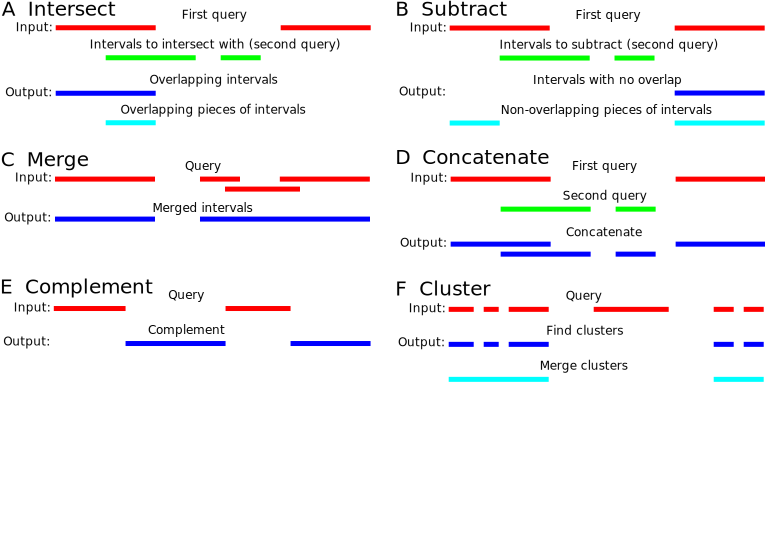
\includegraphics[width=9cm,height=5.5cm]{operation.png}}
  \item intersect,交集:保留重叠的坐标
  \item subtract,减法:去除重叠的坐标
  \item merge,合并:合并重叠的坐标
  \item concatenate,串联:合并多组坐标
  \item complement,补集:取坐标的补集
  \item cluster,聚类:聚合符合要求的坐标
  \item join,联合:根据坐标重叠把两组记录对应起来\textcolor{red}{(与交集的区别)}
\end{itemize}

\vspace*{0.2cm}
\noindent
三、Galaxy简介(10分钟)
\begin{enumerate}
  \item 主界面
  \begin{itemize}
    \item 顶部是刊头:切换“分析数据”、“工作流”和“帐号”等主界面
    \item 左侧栏是工具菜单:以工具集的形式组织罗列着各种工具
    \item 中间是工作区:工具参数设置、使用说明和数据内容、属性等信息的输出位置
    \item 右侧栏是历史面板:以历史记录的形式记录存储着每一步操作
  \end{itemize}
  \item 工具集
  \begin{itemize}
\parpic[fr]{\includegraphics[width=9.5cm]{galaxy.png}}
    \item Get Data:从公共数据库提取数据
    \item Text Manipulation:处理文本数据
    \item Convert Formats:数据格式转换
    \item Operate on Genomic Intervals:坐标的逻辑运算
    \item Statistics和Graph/Display Data:统计绘图
    \item NGS Toolbox:分析第二代测序数据
    \item ……
  \end{itemize}
  \item 学习资料\textcolor{red}{(先易后难,由浅入深)}
  \begin{itemize}
\parpic[fr]{\includegraphics[width=9.5cm]{learnGalaxy.png}}
    \item Galaxy 101
    \item Galaxy Screencasts and Demos
    \item Shared Pages, Histories \& Workflows
    \item Learn Galaxy
    \item Galaxy Wiki
  \end{itemize}
\end{enumerate}

\otherTail
\newpage
\otherHeader

\noindent
四、实验操作(120分钟)

寻找人类基因组(hg19)中22号染色体(chr22)上至少含有10个SNP的外显子。
\begin{enumerate}
  \item 获取数据\textcolor{red}{(选择正确的格式,把结果导出到Galaxy中)}
    \begin{itemize}
      \item 外显子数据:Get Data,UCSC Main,hg19,chr22,RefSeq Genes,BED格式
      \item SNP数据:Get Data,UCSC Main,hg19,chr22,dbSNP137,BED格式
    \end{itemize}
%\parpic[fr]{\includegraphics[width=9cm,height=5cm]{exonSNP.png}}
  \item 提取含有SNP的外显子:Operate on Genomic Intervals,Join\textcolor{red}{(注意数据集的顺序)}
%\vspace*{-0.5cm}
  \item 对外显子上的SNP进行计数:Join,Subtract and Group,Group\textcolor{red}{(注意选择正确的列和需要的操作)}
  \item 筛选至少含有10个SNP的外显子:Filter and Sort,Filter\textcolor{red}{(学习编写筛选表达式)}
  \item 附加外显子的原始信息:Join,Subtract and Group,Compare two Datasets\textcolor{red}{(注意数据集的选择,同时根据每一列的含义选择正确的列)}
  \item 尝试使用不同的工具组合来完成同样的任务,如:Join-Group-Filter-Compare-Sort;Join-Count-Filter-Cut-Sort;Join-Group-Sort-SelectFirst-Join-Cut-Sort\textcolor{red}{(注意不同工具的输出不一样,后续的工具选择和处理过程也会有所差别)}
  \item 尝试对同一物种或其他物种的不同染色体或全基因组进行类似的分析\textcolor{red}{(提示:从历史记录中提取出工作流,修改参数和输入后进行工作流的重运行;学习工作流的使用,了解工作流的优势)}
\end{enumerate}

\begin{figure}[ht]
  \centering
  \includegraphics[width=15cm]{exonSNP.png}
\end{figure}


\otherTail


\end{document}

